\section{Methodology}

\subsection{Energy Balance Solution}

In order to first implement the acoustic energy evolution equation (\ref{eq:dedt}) into iSALE, the acoustic energy density was converted to an energy per unit mass, using $\mathcal{E}_{v}=E/\rho$ \citep{collins2003acoustic}:

\begin{equation}\label{eqdedtmass}
\frac{d \mathcal{E}_{v}}{d t} = \frac{\xi}{4} \nabla^{2}\mathcal{E}_{v} - \frac{c_{p}}{\lambda Q}\mathcal{E}_{v} + e \frac{\tau \dot{\epsilon}}{2\rho}.\vspace{0.2cm}
\end{equation}

This is necessary, as iSALE stores specific energy rather than energy density.

To satisfy the conservation of energy, the energy available for regeneration of acoustic vibrations must be removed from the internal energy of the rock material. In iSALE, the rate of change of internal energy per unit mass, $I$, is given as \citep{collins2002numerical}:

\begin{equation}\label{eq:iSaleInternalEnergy}
\frac{d \left( \rho I\right)}{d t} =\frac{d \left(p + q\right)}{d t} + \tau \dot{\epsilon},\vspace{0.2cm}
\end{equation}

where the terms on the right hand side represents the work done against compression and deformation, respectively. To account for energy transfer, both the acoustic energy lost in heat dissipation and the amount of distortional energy available for acoustic regeneration must be included in equation \ref{eq:iSaleInternalEnergy}. This was achieved by adding the second term and one minus the third term from equation \ref{eqdedtmass} to equation \ref{eq:iSaleInternalEnergy} \citep{collins2002numerical}:

\begin{equation}\label{eq:iSaleInternalEnergyAcoustic}
\frac{d \left(\rho I\right)}{d t} =\frac{d \left(p + q\right)}{d t} + \tau \dot{\epsilon}\left(1-\frac{e}{2}\right)+\frac{c_{p}}{\lambda Q}\mathcal{E}_{v}.\vspace{0.2cm}
\end{equation}

Finally, the first term from equation \ref{eqdedtmass} must also be included to account for the scattering of acoustic energy \citep{collins2002numerical}. This is simply diffusion of acoustic energy, as governed by the Laplace equation:

\begin{equation} \label{eq:xydiff}
\frac{d \mathcal{E}_{v} }{d t} = \frac{\xi}{4} \left( \frac{d^{2} \mathcal{E}_{v}}{d x^{2}} +\frac{d^{2} \mathcal{E}_{v}}{d y^{2}} \right),\vspace{0.2cm}
\end{equation}

or, for a cylindrical coordinate system with angular symmetry about the z-axis;

\begin{equation} \label{eq:cyldiff}
\frac{d \mathcal{E}_{v} }{d t} = \frac{\xi}{4}  \left( \frac{1}{r} \frac{d}{dr} \left( r \frac{d \mathcal{E}_{v}}{dr} \right) + \frac{d^{2} \mathcal{E}_{v}}{dz^{2}}   \right) .\vspace{0.2cm}
\end{equation} 

Equations \ref{eqdedtmass}, \ref{eq:iSaleInternalEnergyAcoustic}, and \ref{eq:cyldiff}, as well as the acoustic fluidisation strength model (equation \ref{eq:yield_vib}) were successfully implemented into the iSALE hydrocode. This is further detailed in \ref{app:modifications}.

Verification of the scatter term subroutine implemented in iSALE was performed using an ideal model. The initial conditions described a sphere of high acoustic energy, surrounded by zero acoustic energy. In this situation, acoustic energy should diffuse/scatter into the sphere's surroundings. The error between the iSALE solution and a second order implicit finite difference solution, computed in Python, for several model resolutions is shown in (Figure \ref{fig:scatter_test}). This demonstrated that the scatter term was successfully implemented, with the iSALE solution showing a greater than first order rate of convergence.

\begin{figure}[!ht]
		\centering
		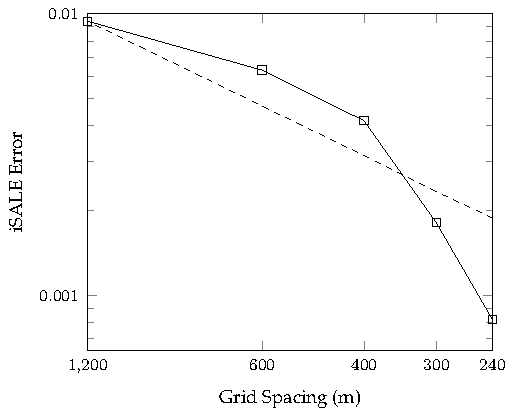
\includegraphics[width=\linewidth]{./images/scatter_test2.pdf}
		%\captionsetup{width=0.58\linewidth}
		\caption{Log-log plot of the error between the implicit finite difference and iSALE solutions to the scattering term in equation \ref{eqdedtmass}, with a test value of $\xi=10^{6}$ m$^2$ s$^{-1}$. The dashed line represents a first order convergence line with a slope of one. As the grid spacing is decreased (i.e., resolution is increased), the iSALE solution shows a greater than first order convergence.\label{fig:scatter_test}}
\end{figure}\vspace{-0.3cm}

\subsection{Models and their Parameters}\label{sec:parameters}

To test the implementation of the Melosh model and contrast its behaviour against the block model, three different sized scenarios of crater formation were created. Both acoustic fluidisation models were applied to each scenario on separate simulations. Table \ref{tb:ABC_table} displays all the acoustic fluidisation parameters used in each scenario, as well as the model setup parameters. Static model parameters are presented in Table \ref{tb:static}. The static strength of rock in each case was assumed to be the same.

\begin{table}[!t]
\small
\centering
\begin{tabular*}{\linewidth}{@{\extracolsep{\fill} }p{3cm} c c c}
\toprule
& \multicolumn{3}{c}{Scenario} \\ \cmidrule{2-4}
Parameter & A & B & C \\ \midrule
Impactor radius, $a$ (km) & 7.200 & 0.720 & 0.072 \\
Impactor resolution & 36 & 24 & 18 \\ 
Grid spacing (m) & 200 & 30 & 4 \\  
Scattering diffusivity, $\xi$ (m$^{2}$ s$^{-1}$) & 10$^3$ & 10$^3$ & 10$^3$ \\
Dissipation quality factor, $Q$ & 10-400 & 10-400 & 10-400 \\
Vibrational wavelength, $\lambda$ (m) & 1440-360 & 144-36 & 14.4-3.6 \\
Regeneration parameter, $e$ & 0.1 & 0.1 & 0.1 \\ \bottomrule
\end{tabular*}
\caption{Melosh model acoustic fluidisation parameters used in each crater formation scenario. Global parameters are given in Table \ref{tb:static}}\label{tb:ABC_table}
\end{table}

\begin{table*}[!bh]
\small
\centering

\begin{tabular*}{\linewidth}{@{\extracolsep{\fill} }p{2cm} l l}
\toprule
Parameter & Description & Value \\ \midrule
$g$ & acceleration of gravity & 9.81 m s$^{-2}$\\
$U$ & impactor velocity & 1.2 $\times$ 10$^{4}$ m s$^{-1}$\\
$T_{\text{melt}}$ & melting temperature & 1673 K \\  
$\mu_{\text{int}}$ & intact material internal coefficient of friction & 2.0 \\
$\mu_{\text{dam}}$ & damaged material internal coefficient of friction  & 0.6\\
$Y_{\text{int}}$& intact material yield strength  & 10$^7$ kg m$^{-1}$ s$^{-2}$\\
$Y_{\text{dam}}$& damaged material yield strength & 10$^4$ kg m$^{-1}$ s$^{-2}$\\
$mat_{\text{t}}$& target material type & granite\\
$mat_{\text{p}}$& impactor material type & granite\\
$\rho_{\text{t}}$ & target material density & 2630 kg m$^{-3}$\\ 
$\rho_{\text{p}}$ & impactor material density & 2630 kg m$^{-3}$ \\  \bottomrule
\end{tabular*}
\caption{Static model parameters used in all Melosh and block model scenarios.}\label{tb:static}
\end{table*}

The square of the compressional wave velocity divided by the shear wave velocity, $\psi$, was maintained at 10 throughout all simulations, following the reasoning provided by \citet{collins2003acoustic}. The single values for $e$ and $\xi$ used here were selected from the range of possible values demonstrated by \citet{collins2003acoustic} in their work simulating the mobility of large rock avalanches. 

The two main parameters that were varied, as shown in Table \ref{tb:ABC_table}, were the vibrational wavelength, $\lambda$, and the quality dissipation factor, $Q$. Both of these are somewhat unconstrained, as are all the parameters in the Melosh model. However, $Q$ has the best constraint as it is similar to another parameter, the seismic $Q$ \citep{melosh1996dynamical}. A typical value of the seismic $Q$ in the upper crust is 500 \citep{anderson1989theory}, which accounts for both elastic energy converted to heat and scattering. In contrast, the Melosh model $Q$ only includes conversion to heat, thus 500 is likely an underestimate. \citet{melosh1999impact}, however, demonstrated that $Q$ must be of the order 10-100 for block model results to realistically fit observed crater profiles. As such, $Q$ was varied between 10-400 in this study. 

The only constraint set on the vibrational wavelength, $\lambda$, is that it must be less than the final crater diameter, but much greater than the material grain size \citep{melosh1979acoustic,collins2002numerical}. In accordance with this, $\lambda$ was assumed to scale proportionally with impactor size \citep{collins2003acoustic}. The block model makes a similar assumption, in that block size is also proportional to impactor size \citep{ivanov1997block}. This assumption is key: if $\lambda$ decreases with decreasing impactor size, the dissipation term in equation \ref{eqdedtmass} will become large, thus acoustic energy will dissipate more rapidly for smaller impacts. Consequently, $\lambda$ was maintained as a fraction of the impactor radius, ranging from $0.2a$ to $0.05a$.

The block model parameters used were similar to typical parameters used in recent work \citetext{e.g., \citet{wunnemann2003numerical}}. 
